\chapter{Bayesian Compressive Sensing}
\label{ch:msce}

In this chapter, we combine the Compressive Sensing framework from Chapter \ref{ch:cs} with the Sparse Bayesian Learning framework from Chapter \ref{ch:rvm} to formulate the \emph{Bayesian Compressive Sensing} (BCS) algorithm.

Following that, we discuss the scenario where the sensing mechanism $\bm\Theta$ corresponds to a signal mask.
We describe how the performance of the BCS algorithm can be boosted via the \emph{Multi-Scale Cascade of Estimations} algorithm.

\section{Compressive Sensing as Linear Regression}
In the Bayesian Compressive Sensing (BCS) \cite{ji2008} framework, we attempt to approach the Compressive Sensing problem from the point of view of linear regression.

Recall the setup from Chapter \ref{ch:cs}.
We are intersted in recovering the signal $\bm v\in\mathbb{R}^M$ from the CS measurements $\bm\Theta\bm v = \bm y\in\mathbb{R}^N$, where $N << M$.
We also assume that $\bm v$ is compressible in the basis $\bm \Psi$.

This means that $\bm w = \bm\Psi^T\bm v$ is well approximated by the $K$-sparse vector $\bm w_K$ which is identical to $\bm w$ for the $K$ elements in $\bm w$ with the largest magnitude.

Thus, $\bm w_e = \bm w - \bm w_K$ is assumed to be very small in magnitude.
Letting $\bm\Phi=\bm\Theta\bm\Psi$, we have
\begin{equation*}
  \bm y = \bm\Theta\bm v = \bm\Theta\bm\Psi\bm w = \bm\Phi\bm w = \bm\Phi\bm w_K + \bm\Phi\bm w_e = \bm\Phi\bm w_K + \bm n_e
\end{equation*}
where $\bm n_e = \bm\Phi\bm w_e$ will be regarded as noise.
Furthermore, there could be an additional noise source $\bm n$ in the CS measurements $\bm y$ (e.g. due to finite precision in the measurement device) so that, overall,
\begin{equation}
\label{eqn:bcs_setup}
  \bm y = \bm\Phi\bm w_K + \bm n_e + \bm n = \bm\Phi\bm w_K + \bm \epsilon
\end{equation}
with $\bm\epsilon = \bm n_e + \bm n$.

In the BCS literature \cite{ji2008}, $\bm\epsilon$ is typically approximated by a zero-mean Gaussian noise variable with an unknown variance $\sigma^2$:
\begin{equation}
\label{eqn:bcs_noise}
  \bm\epsilon\sim\mathcal{N}(0,\sigma^2\bm I_N).
\end{equation}

Although this assumption may not always be completely accurate in practice, it is often used for its desirable analytical properties.
A possible justification is that the sensing matrix $\bm\Theta$ is usually constructed randomly (often using Gaussian samples) and that the noise source $\bm n$ in the CS measurements is typically represented by a zero-mean Gaussian distribution.

Note the similarity between equations (\ref{eqn:bcs_setup}) and (\ref{eqn:bcs_noise}) and the geneneral linear regression model in equations (\ref{rvm:lklhd_2}) and (\ref{rvm:error}).
The only difference is that, in equation (\ref{eqn:bcs_setup}), we have the addtional constraint that $\bm w_K$ is \emph{sparse}.

Since in the BCS framework, we wish to solve the CS problem from a Bayesian standpoint, we are interested in computing a full posterior distribution of the weights $\bm w_K$ and the noise variance $\sigma^2$.
The sparsity constraint can be entered into the model by placing a sparseness-inducing prior distribution over the weights $\bm w_K$.

There is a range of popular sparseness priors.
However, to make the connection to the RVM and exploit the analysis from Chapter \ref{ch:rvm}, we choose the prior (\ref{eqn:prior_w})
\begin{equation*}
  p(\bm w_K\,|\,\bm \alpha) = \prod_{j=1}^M \mathcal{N}\left(w_j\,|\,0,\alpha_j^{-1}\right)
\end{equation*}

To summarize, we solve the CS problem by passing the CS measurements $\bm y$ and the matrix $\bm\Phi$ to train a RVM.
The SBBL algorithm (Algorithm \ref{rvm:alg2}) is then used to compute the posterior distribution of the weights $\bm w \in \mathbb{R}^M$ (\ref{rvm:posterior}).

The desired signal $\bm v\in\mathbb{R}^M$ can then by recovered by computing 
\begin{equation}
  \label{eqn:bcs_recover}
  \bm{\hat v} = \bm\Psi\bm\mu
\end{equation} 
where $\bm \mu$ is the posterior mean of $\bm w$.

The method of applying the RVM to CS inversion is sometimes referred to as the Bayesian Compressive Sensing (BCS) algorithm.
The BCS algorithm was compared against state-of-the-art deterministic CS algorithms by \cite{ji2008,pilikos2014} and shown to give comparable performance.

We have implemented the BCS algorithm as part of our Compressive Sensing algorithm.
Using BCS, our implementation is able to reconstruct video signals from a small number of CS measurements that were sampled by a general sensing mechanism $\bm\Theta$. 


\section{The Case when \texorpdfstring{$\bm\Theta$}{[Theta]} is a Signal Mask}

\subsection{Image Interpolation}
\begin{figure}
  \centering
  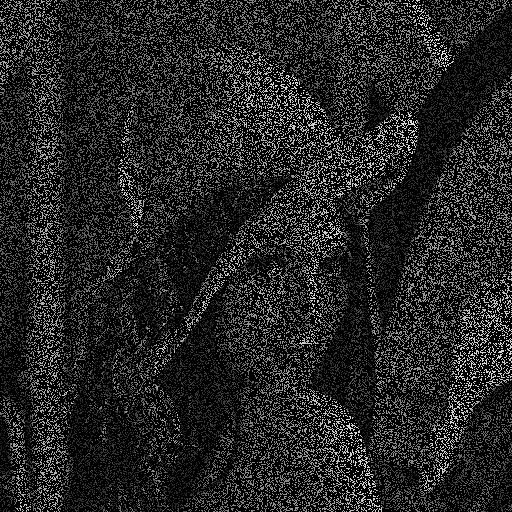
\includegraphics[width=0.6\textwidth]{Chapter5/Images/lenna_MASKED.png}
  \caption[Example of masked image signal]{Example of an image with missing pixel values. The missing data points are set to zero and displayed in black}
  \label{fig:lenna_mask}
\end{figure}

If the sensing matrix $\bm\Theta$ is a signal mask (see Section \ref{sect:sensors}), the CS measurements $y$ of an image $\bm v$ can be visualized as an image with missing pixel values as in Figure \ref{fig:lenna_mask}.
The problem of reconstructing such signals is sometimes referred to as \emph{interpolation}.

In this context, the design matrix $\bm\Phi$ can be computed efficiently from $\bm\Psi$ by simply deleting all the rows in $\bm\Psi$ that correspond to the entries of $\bm v$ that have missing data.

Moreover, it is possible to get a slight performance boost in the reconstruction by filling in the BCS solution $\bm{\hat v}$ (\ref{eqn:bcs_recover}) with the measured at data $\bm y$ at the appropriate locations.

\subsection{Reconstruction using Haar Wavelets}
Using the BCS model from above with a Haar basis matrix, we reconstruct the image in Figure \ref{fig:lenna_mask}.
We display the output in Figure \ref{fig:lenna_rvm} for various scales of the Haar basis.
\begin{figure}
\centering
  \begin{subfigure}{0.4\textwidth}
    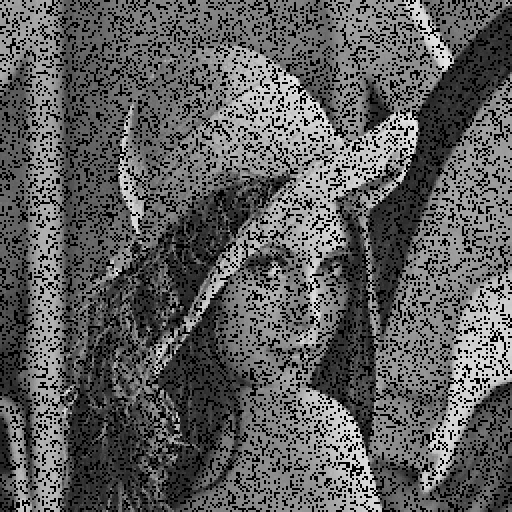
\includegraphics[width=\textwidth]{Chapter5/Images/lenna_haar1.png}
    \caption{Scale 1: PSNR = 11.75}
  \end{subfigure}
  \begin{subfigure}{0.4\textwidth}
    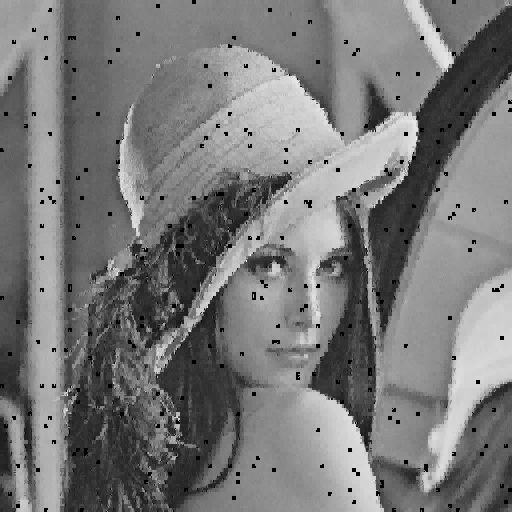
\includegraphics[width=\textwidth]{Chapter5/Images/lenna_haar2.png}
    \caption{Scale 2: PSNR = 21.78}
  \end{subfigure}
  \begin{subfigure}{0.4\textwidth}
    
\includegraphics[width=\textwidth]{Chapter5/Images/lenna_haar3.png}
    \caption{Scale 3: PSNR = 24.15}
  \end{subfigure}
  \begin{subfigure}{0.4\textwidth}
    
\includegraphics[width=\textwidth]{Chapter5/Images/lenna_haar4.png}
    \caption{Scale 4: PSNR = 23.72}
  \end{subfigure}  
  \caption[Reconstruction of masked image signals using Haar wavelets at various scales]{Reconstruction if the image in Figure \ref{fig:lenna_mask} using the RVM with Haar wavelets at various scales.
    We use the \emph{Peak Signal-to-Noise Ratio (PSNR)} as our performance metric. The larger the PSNR, the more accurate the reconstruction. See Chapter \ref{ch:results} for a definition of the PSNR.}
  \label{fig:lenna_rvm}
\end{figure}

We see that the scale of the wavelet basis has a strong effect on the quality of the reconstruction.
Wavelets at lower scales can fail to reconstruct the entire image, but generally give a more accurate reconstruction at the portion of the image where they succeed.
On the other, wavelets at larger scales typically achieve a reconstruction of the entire image at the cost of increased blurring or pixelation.
This conflict can be seen in Figure \ref{fig:lenna_rvm} by contrasting panel (c) with panel (d):
They both achieve a reconstruction of the entire image, but scale 3 outperforms scale 4 in this example.
Moreover, if we compare panel (b) with panel (d), we see that, in the part of the image where the recovery succeeds, the scale 2 reconstruction manages to recover finer details than both scale 3 and scale 4.

To explain why this tradeoff exists, recall that two-dimensional Haar wavelets at scale $s$ have a support of size up to $2^s\times 2^s$.
Thus, at small scales, the support of the individual basis functions is small.
For example, suppose $s=1$.
In this case, each Haar basis functions covers an area of $2\times 2$ pixels (see Figure \ref{fig:haar2_basis}).
Using these wavelets, we can capture very local relationships between the pixels.
This allows us to recover finer details in the reconstruction.

However, it can also lead to the formation of black pixels.
At scale 1, each column $j$ of the Haar basis matrix $\bm \Psi$ contains exactly 4 non-zero entries corresponding to the four pixel locations that are covered by the $j$th basis function.
If the masked image happens to be missing data at all four of these locations, the corresponding rows of the basis matrix $\bm\Psi$ will be deleted when forming the design matrix $\bm\Phi=\bm\Theta\bm\Psi$.
Therefore, column $j$ of the design matrix will be zero.
The same is true for the three columns that correspond to the remaining locations that were covered by basis function $j$.

The SSBL algorithm will generally not select any columns that are completely zero, since they offer no change to the marginal likelihood.
The consequence is that the corresponding entries in the posterior mean $\bm\mu$ of $\bm w$ will remain zero.
The resulting reconstruction (\ref{eqn:bcs_recover}) will therefore be unable to recover the $2\times 2$ patch covered by basis function $j$.

This problem can be mitigated by using larger scales since, for any given total number of missing pixels, it is less likely that larger square patches of the masked image are completely void of data.
However, the SSBL Algorithm generally prefers to add basis functions with larger support to the model, since they typically cause a larger increase in the Marginal Likelihood.
The result is that we get a more blurred reconstruction and lose the finer details, even in parts of the image that would have been accurately recovered at smaller scales.





\subsection{Multi-Scale Cascade of Estimations Algorithm}
The \emph{Multi-Scale Cascade of Estimations} (MSCE) algorithm was developed by \cite{pilikos2014} to this tradeoff between inaccurate but complete reconstructions and accurate but incomplete reconstructions.

To explain the algorithm, note that, in the interpolation problem, the BCS reconstruction (\ref{eqn:bcs_recover}) is equivalent to computing the mean (\ref{rvm:pred_mean}) of the predictive distribution (\ref{rvm:predictive}) of the entire signal $\bm v$.
Moreover, we can compute the predictive variance (\ref{rvm:pred_var}) (or error-bars) for each estimate:
\begin{equation}
\label{eqn:msce_error}
  (\sigma^2)^* = \sigma^2 +\bm\psi(\bm x^*)^T\bm\Sigma\bm\psi(\bm x).
\end{equation}

The MSCE algorithm uses these error bars to construct a cascade of BCS algorithms, that builds up the scale of the Haar wavelets.

We begin by executing the BCS algorithm using Haar wavelets at the first scale.
Next, we compute equation (\ref{eqn:msce_error}) for each location in the signal in which originally had missing data.
If $(\sigma^2)^*$ is small, but larger than the noise variance $\sigma^2$, we trust the estimate and accept it. 
If $(\sigma^2)^*$ is large, we do not trust the estimate and reject it.

If $(\sigma^2)^*$ is equal to $\sigma^2$, then $\bm\psi(\bm x^*)^T\bm\Sigma\bm\psi(\bm x^*) = 0$. 
This means that $\bm\psi(\bm x^*) = 0$ since, by postive definiteness of $\bm\Sigma$, $\bm\psi(\bm x^*)^T\bm\Sigma\bm\psi(\bm x^*) > 0$ unless $\bm\psi(\bm x^*) = 0$.
Thus, the RVM predicted the pixel value at location $\bm x^*$ to be zero. 
Since the recovery of the pixel was unsuccessful in this case, we reject the estimate.

The output of the current cascade becomes the target vector of the next cascade.
The new basis matrix is constructed using Haar wavelets that are one scale higher than in the previous cascade.

This process it repeated until we no more signal values marked as missing, or until some pre-defined maximum for the scale of the Haar basis is reached.

We have summarized the MCSE in Algorithm \ref{alg3}.

\begin{algorithm}
  \caption{Multi-Scale Cascade of Estimations \cite{pilikos2014}}
  \label{alg3}
  \begin{algorithmic}[1]
    \State Set $s=1$
    \State Let $\bm y_1 = \bm y$
    \While {$s \leq s_{max}$}
    \State Form basis matrix $\bm\Psi$ using Haar wavelets at scale $s$
    \State Call Sequential Sparse Bayesian Learning Algorithm with target
    \Statex $\qquad$ vector $\bm y_j$ and design matrix $\bm\Phi=\bm\Theta\bm\Psi$ to get the estimate $\bm{\hat v}_s$
    \State Compute $(\sigma^2)^*$ for all newly reconstructed pixel values using equation (\ref{eqn:msce_error})
    \State If $(\sigma^2)^* = \sigma^2$ or $(\sigma^2)^* > \tau$, discard the corresponding estimate
    \State Set $s = s+1$
    \State Let $\bm y_s$ be $\bm{\hat v}_s$ after the discarded estimates are deleted
    \EndWhile
    \State\Return $\bm v = \bm y_s$
  \end{algorithmic}
\end{algorithm}

